\documentclass{article}

\usepackage[brazil]{babel}
\usepackage[utf8]{inputenc}
\usepackage[T1]{fontenc}% optional T1 font encoding
\usepackage[%
    colorlinks=true,
    pdfborder={0 0 0},
    linkcolor=red
]{hyperref}
\usepackage[all]{hypcap}
\usepackage{amsmath}
\interdisplaylinepenalty=2500
\usepackage{graphicx}
\usepackage[cmintegrals]{newtxmath}
\usepackage{cite}
\usepackage{listings}
\usepackage{hyperref}
\usepackage{indentfirst}
\usepackage{siunitx}
\usepackage{textgreek}
\usepackage[portuguese,linesnumbered,ruled]{algorithm2e}
\usepackage{multirow}
\usepackage{anysize}
\usepackage{float}
\usepackage{aliascnt}
\newaliascnt{eqfloat}{equation}
\newfloat{eqfloat}{h}{eqflts}
\floatname{eqfloat}{Equation}

\newcommand*{\ORGeqfloat}{}
\let\ORGeqfloat\eqfloat
\def\eqfloat{%
  \let\ORIGINALcaption\caption
  \def\caption{%
    \addtocounter{equation}{-1}%
    \ORIGINALcaption
  }%
  \ORGeqfloat
}

\begin{document}

    \title{Exp. IV — transístores BJT e Buffer de Tensão}
    \author{Bianca Yoshie Itiroko - 164923, Luiz Eduardo Cartolano - 183012, Seong Eun Kim - 177143 \\ EE534 - Turma Y - Grupo 2}
    \date{Outubro de 2018}
    
    \maketitle
    
    \begin{abstract}
        Este experimento tem como objetivo estudar a influência de um estágio de saída com um transístor do tipo de junção bipolar (BJT) no estágio de pré-amplificação. Nessa configuração, foi possível obter o ganho de tensão de $12,97 V/V$. Ao final do experimento, será possível amplificar o sinal de um microfone de eletreto para reproduzi-lo em um alto-falante.
    \end{abstract}
    
    \section{Introdução}
        O transístor de junção bipolar, \emph{BJT}, é o tipo de transístor mais comum presente no mercado, devido a sua facilidade de polarização e durabilidade. Seu nome se dá fruto do seu processo de condução, que é realizado por dois tipos de carga - positiva (lacunas) e negativa (elétrons).  São normalmente compostos de três terminais, sendo os eles, a Base, o Emissor(\emph{Emitter}) e o Coletor(\emph{Collector}). Existem essencialmente dois tipos de \emph{BJT}, o do tipo NPN e PNP. Os transístores \emph{BJT} tem uma série de aplicações práticas no nosso dia a dia, sendo especialmente usados como amplificadores de corrente(ou tensão) e como controle \emph{ON-OFF}(chaves do tipo liga-desliga).
    
        Um buffer de tensão, é um amplificador de ganho unitário usado para isolar e conectar um estágio de alta impedância de entrada a uma carga de baixa impedância de saída. Ele é usualmente chamado de seguidor de tensão, já que esse circuito faz uma cópia da tensão em sua entrada na sua saída.
    
        Neste experimento, será estudado, com mais detalhes, as características do \emph{BJT}, e também, o seu uso no projeto de um seguidor de emissor. Busca-se entender as relações entre as tensões do transístor de modo que ele seja polarizado e, ao fim do experimento, almeja-se criar um circuito capaz de amplificar o sinal de um microfone de eletreto para reproduzi-lo em um alto-falante.
    
    \section{Procedimentos}
        Para a realização dos experimentos propostos, foram utilizados os seguintes componentes e ferramentas: Osciloscópio digital de dois canais, gerador de ondas/funções, fonte de tensão contínua, cabos com plugs banana e coaxial, multímetro digital, placa de contatos, transístores \emph{BSS100 e 2N2222}, um resistor de potência de $100\Omega (5W)$ e um de $56\Omega (5W)$, capacitores de $680nF$ e $220nF$, resistores de $82\Omega$, $6,8k\Omega$ $1M\Omega$ e $3,9M\Omega$. Além de um alto-falante e um microfone de eletreto.
    
        A primeira parte consiste na familiarização dos alunos com o \emph{BJT}, para isso montou-se o circuito que pode ser observado na Figura \ref{fig:circLab4}. Nesta etapa buscou-se encontrar a tensão "limiar" do transístor, V$_{BE}$. Para isso mediu-se as tensões $V_B$ e $V_E$, também avaliou-se o ganho de tensão do circuito. Um detalhe importante ao qual deve-se atentar nesse momento é a presença do resistor de potência, e também a tensão de V$_{CC}$ (corrente contínua), já que em valores muito altos ela pode queimar o transístor.
    
        Na segunda etapa do laboratório, buscou-se estudar uma das aplicações práticas do transístor. Para isso, projetou-se um circuito capaz de amplificar o sinal de um microfone de eletreto para reproduzi-lo em um alto-falante. Para isso, acoplou-se o circuito da Figura \ref{fig:circLab4} ao circuito da Figura \ref{fig:circLab3}. Novamente, deve-se reiterar o cuidado com a tensão contínua V$_{CC}$ e com o posicionamento dos canais do transístor no circuito, afinal, esses pequenos detalhes são fundamentais para garantir a integridade do circuito.
    
    \section{Discussão}
        Na primeira parte do experimento usou-se o circuito da Figura \ref{fig:circLab4}, junto a uma tensão contínua $V_{CC}$ de 12V e com o gerador de funções desligado, para medir as tensões de V$_B$ e V$_E$. A partir dos valores calculados foi possível calcular alguns parâmetros interessantes para avaliar o comportamento do transístor \emph{BJT}. A partir da Equação \ref{eq:Ib} pudemos encontrar o que a corrente que chega ao terminal base era de $1,16 mA$. Usando a Equação \ref{eq:Ie} foi possível encontrar a corrente que flui pelo emissor, e uma vez que a conhecíamos, pode-se usar a Equação \ref{eq:Ic} para encontrar a corrente que chegava ao coletor, a qual apresentou valor de $0,13A$. Ainda usando os valores de tensão, pode-se calcular a tensão existente entre a base e o emissor do \emph{BJT}, esta funciona como uma espécie de tensão limiar para a qual o transístor começa a operar, o valor empírico encontrado para ela foi de $0,595V$, enquanto que o valor encontrado caso fosse usada a Equação \ref{eq:Vbe} seria de $0,73V$, essa pequena diferença é provavelmente fruto da baixa precisão do     multímetro. Usando a corrente do coletor, pode-se encontrar outro importante parâmetro do transístor, a sua transcondutância, que é a taxa de variação da corrente na porta de saída em relação à tensão aplicada na porta de entrada, para tal cálculo usa-se a Equação \ref{eq:transcondutancia}, encontrando um valor de $5 A / V$. 
        
        Após determinar tais valores, ainda visando conhecer melhor o funcionamento do circuito montado, ligou-se o gerador de funções, com uma onda senoidal. A relação entre as tensões de entrada e saída podem ser observadas na Figura \ref{fig:NewFile1}. Analisando a tensão de entrada e saída, podemos perceber que o ganho de tensão obtido experimentalmente foi de $A_v = 0,98 V / V$, enquanto que ao usar a Equação \ref{eq:ganho_tensao} obtemos um valor teórico de $A_v = 0,99 V / V$, o que indica um bom funcionamento do nosso amplificador. Um fato interessante de se observar do circuito amplificador em questão, é que ele não amplifica a tensão de entrada, mas ainda assim, possui uma série de aplicações práticas.
    
        Após esse primeiro momento, acoplamos os circuitos das Figuras \ref{fig:circLab3} e \ref{fig:circLab4}, a fim de analisar os estágios parciais e total de amplificação. Para o primeiro estágio, estágio de pré-amplificação (saída do circuito da Figura \ref{fig:circLab3}), obteve-se um ganho de $8,44 V / V$. Se compararmos com o ganho obtido no ultimo experimento, vide \cite{ref:exp3}, é possível observar que ele se mantém praticamente o mesmo, logo acoplar o circuito não alterou suas características. Para o segundo estágio (relacionado ao circuito da Figura \ref{fig:circLab4}), obteve-se um ganho de $0,98 V / V$. Já o ganho total de ambos os circuitos acoplados foi de $12,97 V / V$, o que é um fator considerável.
        
        Visando eliminar a tensão contínua e manter só a oscilação, colocou-se um capacitor de acoplamento e acoplou-se o alto-falante na saída do estágio. Então, usou-se o osciloscópio e mediu-se o ganho do primeiro estágio, que foi de $1,54V/V$ (vide Figura \ref{fig:NewFile10}), do segundo estágio, de $0,45V/V$ (vide Figura \ref{fig:NewFile8}), e o ganho total, de $1,49V/V$ (vide Figura \ref{fig:NewFile9}). Observa-se que quando colocou-se o alto-falante o ganho diminuiu, pois ele adiciona uma resistência ao circuito.
        
        Para a última parte do experimento, acoplou-se um microfone de eletreto à entrada do estágio fonte-comum e visando analisar a saída do mesmo e do amplificador, conectou-se o osciloscópio. Assim que o sinal de entrada começou a passar, verificou-se que havia som no alto-falante, indicando o sucesso da etapa. Ao medir a amplitude do sinal de entrada em relação à saída, obteve-se o ganho de tensão de 2,52.
        
        Idealmente, as ondas deveriam ter a mesma frequência, entretanto há distorções devido a mal contato dos fios e pelo fato de os componentes usados não serem ideais.
        
        No osciloscópio pode-se ver a Figura \ref{fig:circuitoMicro} e ao analisá-la, vê-se que há uma amplificação no sinal. O microfone coleta ondas acústicas, transforma-as em ondas elétricas e as envia para o alto-falante. Este as amplifica e as transforma em onda acústica novamente.
        
        O circuito usado nesta última parte é bastante interessante, em especial pela maneira como seus blocos são estruturados a fim de obter o resultado desejado. Pode-se dividi-lo em dois blocos, cada qual com sua função específica, o primeiro bloco (observado na Figura \ref{fig:circLab3}), é um estágio de pré-amplificação, com uma alta impedância de entrada, ele é responsável por receber um sinal e amplificá-lo, a fim de acionar a segunda parte. Esta (observada na \ref{fig:circLab4}) precisa ser capaz de apresentar a maior tensão para a saída com baixa impedância, a fim de que essa possa ser usada pelo próximo dispositivo (por exemplo, alto-falantes). Isso é essencialmente alcançado por um circuito que pode fornecer a tensão da seção anterior com uma corrente muito mais alta do que a que estaria disponível na fonte de sinal original (características da topologia do seguidor de emissor, como pode-se ver com mais detalhes em \cite{Sedra2004}).
    
    \section{Conclusão}
        Neste experimento buscou-se estudar o comportamento do transístor \emph{BJT} e também de um circuito amplificador que, acoplado a um estágio de pré-amplificação é capaz de transformar ondas acústicas em elétricas e depois retransmiti-las em forma de ondas acústicas. 
        
        Para a primeira parte, obteve-se resultados consideravelmente bons e bem próximos ao esperado. As pequenas diferenças entre valores empíricos e teóricos são provavelmente em decorrência da baixa qualidade dos cabos e resistências e, a fim de melhorar em uma próxima iteração, poderia-se usar elementos mais precisos, e também usar um sistema de medição de valores com maior precisão.
        
        Para a segunda parte, montou-se o circuito amplificador, para o qual obteve-se ganhos condizentes com o esperado, o que torna possível concluir sucesso na montagem dos mesmos. O único porém foi que observou-se, que o circuito gerava bastante ruído, ao conectar-se o microfone. Uma forma de melhorar os resultados seria usando cabos menos desgastados.
    
    \nocite{*}
    \bibliographystyle{plain}
    \bibliography{references}
    
    \newpage
    \section*{Anexos}
    
    %%%%%%%%%%%%%%%%%
    %   EQUAÇÕES    %
    %%%%%%%%%%%%%%%%%
    \begin{eqfloat}[h!]
        \begin{equation}
            A_v = \frac{R_E}{R_E + g_m^{-1}}
            \label{eq:ganho_tensao}
        \end{equation}
        \caption{Ganho de tensão do transístor \emph{BJT}.}
    \end{eqfloat}
    
    \begin{eqfloat}[h!]
        \begin{equation}
            g_m = \frac{I_C}{V_T}
            \label{eq:transcondutancia}
        \end{equation}
        \caption{Transcondutância do transístor \emph{BJT}.}
    \end{eqfloat}
    
    \begin{eqfloat}[h!]
        \begin{equation}
            V_{BE} = V_B - V_E
            \label{eq:Vbe}
        \end{equation}
        \caption{Tensão entre o terminal da base e do emissor no transístor \emph{BJT}.}
    \end{eqfloat}
    
    \begin{eqfloat}[h!]
        \begin{equation}
            i_b = \frac{V_{CC} - V_B}{R_B}
            \label{eq:Ib}
        \end{equation}
        \caption{Corrente que entra no terminal base do transístor \emph{BJT}.}
    \end{eqfloat}
    
    \begin{eqfloat}[h!]
        \begin{equation}
            i_c = (\frac{\beta}{\beta + 1}) \cdot i_e
            \label{eq:Ic}
        \end{equation}
        \caption{Corrente que entra no terminal coletor do transístor \emph{BJT}.}
    \end{eqfloat}
    
    \begin{eqfloat}[h!]
        \begin{equation}
            i_e = \frac{V_E}{R_E}
            \label{eq:Ie}
        \end{equation}
        \caption{Corrente que sai do emissor do transístor \emph{BJT}.}
    \end{eqfloat}
    
    
    %%%%%%%%%%%%%%
    %   FIGURAS  %
    %%%%%%%%%%%%%%
    
    \begin{figure}[h!]
        \centering
        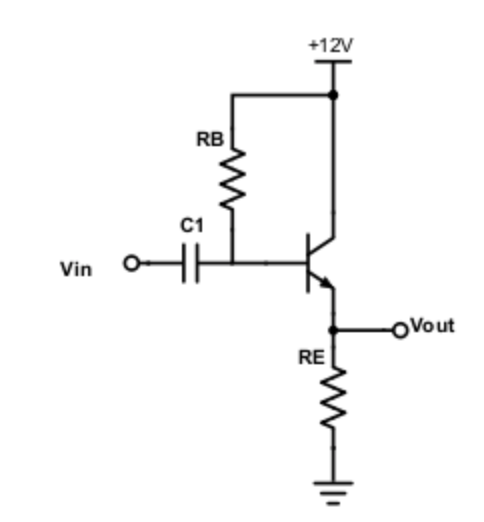
\includegraphics[height=5.5cm]{imgSource/circuitolab4.png}
        \caption{Circuito seguidor de emissor com transístor BJT.}
        \label{fig:circLab4}
    \end{figure}
    
    
    \begin{figure}[h!]
        \centering
        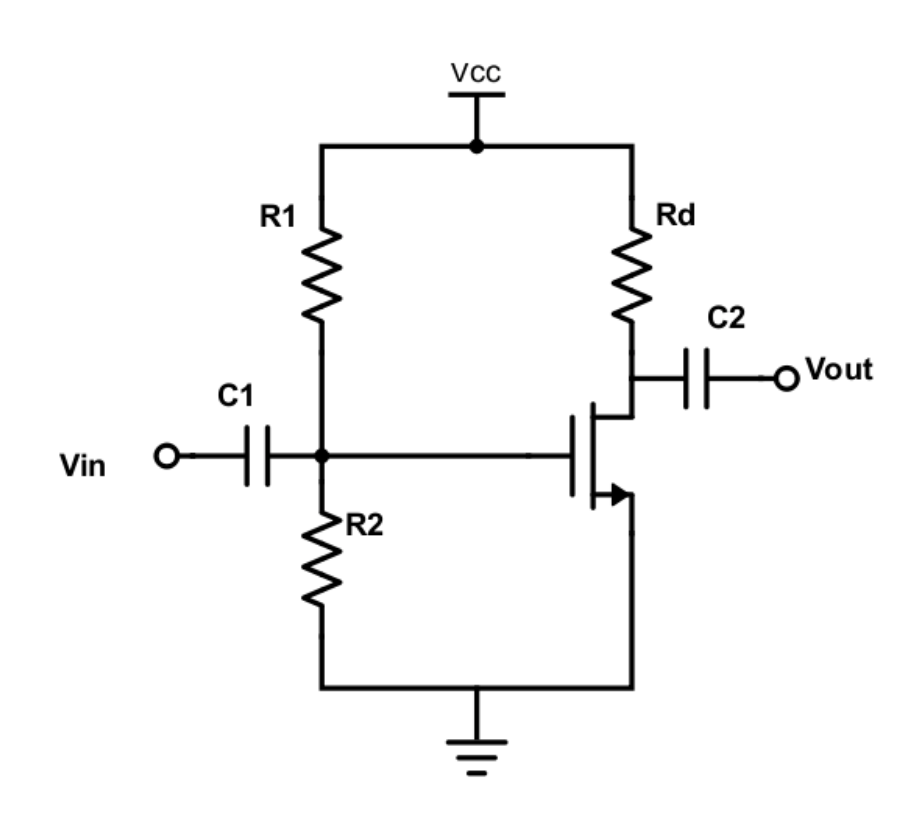
\includegraphics[height=5.5cm]{imgSource/circuitolab3.png}
        \caption{Circuito amplificador do laboratório passado.}
        \label{fig:circLab3}
    \end{figure}
    
    \begin{figure}[h!]
        \centering
        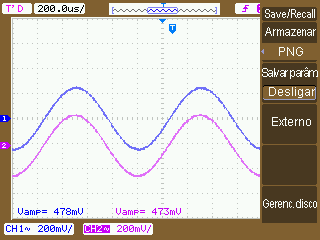
\includegraphics[height=5.5cm]{imgSource/NewFile1.png}
        \caption{Ganho de tensão do circuito seguidor de emissor.}
        \label{fig:NewFile1}
    \end{figure}
    
    \begin{figure}[h!]
        \centering
        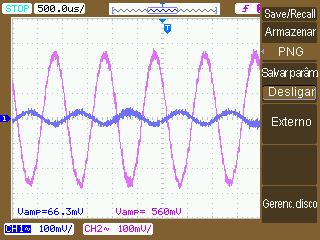
\includegraphics[height=5.5cm]{imgSource/NewFile2.png}
        \caption{Ganho de tensão no primeiro estágio do circuito acoplado.}
        \label{fig:NewFile2}
    \end{figure}
    
    \begin{figure}[h!]
        \centering
        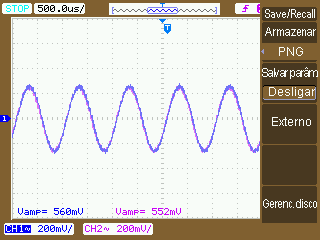
\includegraphics[height=5.5cm]{imgSource/NewFile3.png}
        \caption{Ganho de tensão no segundo estágio do circuito acoplado.}
        \label{fig:NewFile3}
    \end{figure}
    
    \begin{figure}[h!]
        \centering
        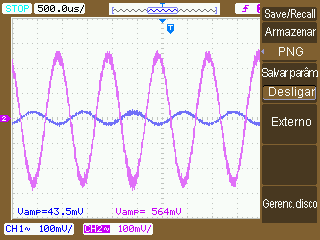
\includegraphics[height=5.5cm]{imgSource/NewFile4.png}
        \caption{Ganho de tensão total do circuito acoplado.}
        \label{fig:NewFile4}
    \end{figure}
    
    \begin{figure}[h!]
        \centering
        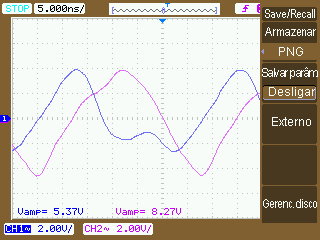
\includegraphics[height=5.5cm]{imgSource/NewFile10.png}
        \caption{Ganho de tensão no primeiro estágio do circuito acoplado a uma caixa de som.}
        \label{fig:NewFile10}
    \end{figure}
    
    \begin{figure}[h!]
        \centering
        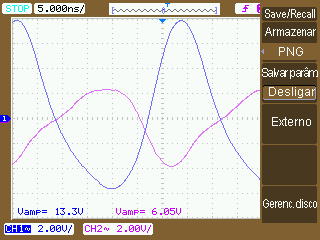
\includegraphics[height=5.5cm]{imgSource/NewFile8.png}
        \caption{Ganho de tensão no segundo estágio do circuito acoplado a uma caixa de som.}
        \label{fig:NewFile8}
    \end{figure}
    
    \begin{figure}[h!]
        \centering
        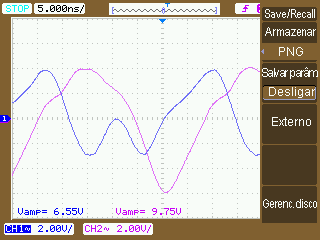
\includegraphics[height=5.5cm]{imgSource/NewFile9.png}
        \caption{Ganho de tensão total do circuito acoplado a uma caixa de som.}
        \label{fig:NewFile9}
    \end{figure}
    
    \begin{figure}[h!]
        \centering
        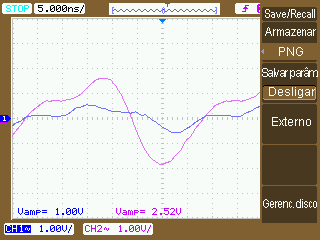
\includegraphics[height=5.5cm]{imgSource/NewFile11.png}
        \caption{Canais do osciloscópico quando se usa um microfone de eletreto como entrada no primeiro estágio.}
        \label{fig:NewFile11}
    \end{figure}
    
    \begin{figure}[h!]
        \centering
        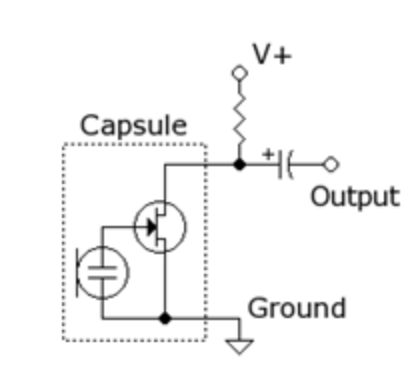
\includegraphics[height=5.5cm]{imgSource/circuitoMicro.png}
        \caption{Esquema de polarização do microfone de eletreto. O terminal negativo do microfone é aquele ligado à carcaça.}
        \label{fig:circuitoMicro}
    \end{figure}

\end{document}